% Figure s06f06_dispersion (Session 6): ferromagnetic against antiferromagnetic magnons.
% The image is rendered by figures/blender/s06f06_dispersion.py; the coordinates of the labels come from
% figures/blender/out/s06f06_dispersion*_anchors.tex. Build with figures/blender/build_figure.sh s06f06_dispersion.
\documentclass[11pt,tikz,border=0pt]{standalone}
\usepackage[T1]{fontenc}
\usepackage{amsmath,amssymb,graphicx,bm}
\usepackage{xcolor}
\usetikzlibrary{arrows.meta,calc}
% The three label colors of the figures, with the same values as in src/figures_preamble.tex.
\definecolor{aqmaccent}{RGB}{31,78,121}
\definecolor{aqmbroken}{RGB}{168,42,34}
\definecolor{aqmmuted}{RGB}{125,125,125}

% Shared TikZ styles of the overlays: axis arrows drawn on top of the renders, between anchors
% written by the scripts, so that they can be adjusted without rendering again.
\tikzset{
  axarrow/.style={line width=0.6pt, draw=black!70, -{Stealth[length=4.5pt,width=3.5pt]}},
  axlbl/.style={font=\small, inner sep=1.5pt},
}
% A discrete color key: \aqmkey{(x,y)}{color 1}{label 1}{color 2}{label 2} draws two swatches in a
% column with their labels, anchored at its north west corner. The colors are the sRGB values
% used in the render, defined below.
\definecolor{keypos}{RGB}{118,158,198}
\definecolor{keyneg}{RGB}{214,150,132}
\definecolor{keyup}{RGB}{224,62,40}
\definecolor{keydown}{RGB}{40,92,200}
\definecolor{keydark}{RGB}{31,78,121}
\definecolor{keylight}{RGB}{118,158,198}
\newcommand{\aqmkey}[5]{%
  \begin{scope}[shift={#1}]
    \fill[#2, draw=black!40, line width=0.3pt] (0,-0.32) rectangle (0.32,0);
    \node[font=\small, anchor=west, inner sep=1.5pt] at (0.38,-0.16) {#3};
    \fill[#4, draw=black!40, line width=0.3pt] (0,-0.74) rectangle (0.32,-0.42);
    \node[font=\small, anchor=west, inner sep=1.5pt] at (0.38,-0.58) {#5};
  \end{scope}}
% The same key in one row, for a figure with no room for a column.
\newcommand{\aqmkeyrow}[5]{%
  \begin{scope}[shift={#1}]
    \fill[#2, draw=black!40, line width=0.3pt] (0,-0.32) rectangle (0.32,0);
    \node[font=\small, anchor=west, inner sep=1.5pt] (k1) at (0.38,-0.16) {#3};
    \fill[#4, draw=black!40, line width=0.3pt] ([xshift=0.25cm]k1.east |- 0,-0.32) rectangle ++(0.32,0.32);
    \node[font=\small, anchor=west, inner sep=1.5pt] at ([xshift=0.63cm]k1.east) {#5};
  \end{scope}}

\newlength{\figw}\setlength{\figw}{12.50cm}   % 0.80 of the text width, before the empty margins of the render are cropped

\begin{document}
\begin{tikzpicture}[lbl/.style={font=\small, inner sep=1.5pt}, pnl/.style={font=\small\bfseries, inner sep=1.5pt}]
  \begin{scope}[shift={(0.00cm,0.00cm)}]
    \setlength{\figw}{8.30cm}
    \node[overlay, anchor=south west, inner sep=0pt] at (0,0)
      {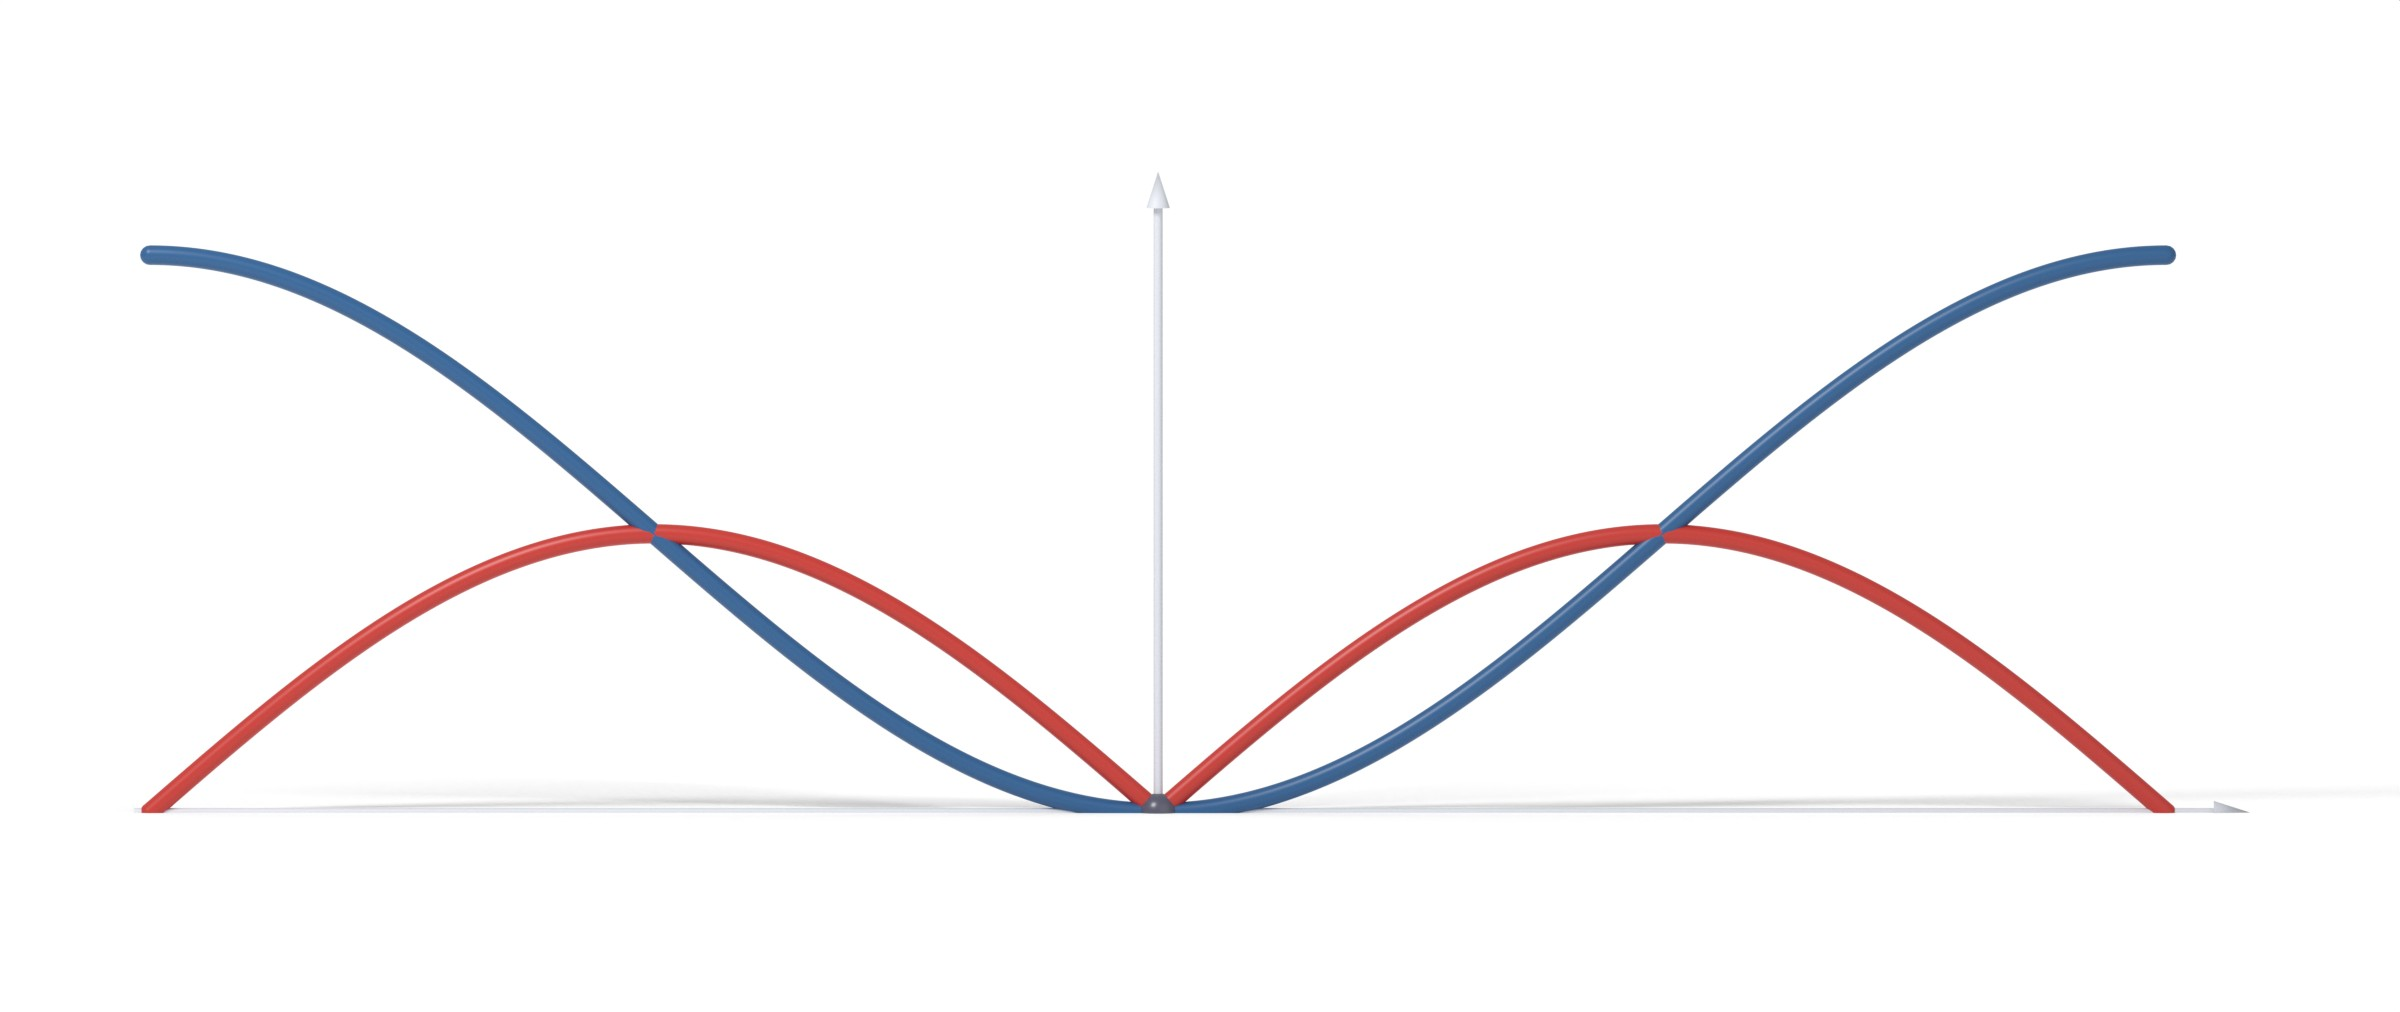
\includegraphics[width=\figw]{../blender/out/s06f06_dispersion_main.jpg}};
    % written by build_figure.sh; the painted part of the image
\path (0.0554\figw,0.0817\figw) rectangle (0.9925\figw,0.3500\figw);

    %% written by figlib.py; x and y in units of the image width
\coordinate (maink) at (0.9375\figw,0.0831\figw);
\coordinate (mainE) at (0.4826\figw,0.3502\figw);
\coordinate (mainkmax) at (0.9027\figw,0.0796\figw);
\coordinate (mainkmin) at (0.0625\figw,0.0796\figw);
\coordinate (mainfm) at (0.7430\figw,0.2420\figw);
\coordinate (mainafm) at (0.6086\figw,0.1770\figw);
\coordinate (mainpanel) at (0.0625\figw,0.3560\figw);

    \node[lbl, anchor=west] at (maink) {$ka$};
    \node[lbl, anchor=west] at (mainE) {$E/|J|Sz$};
    \node[lbl, anchor=north] at (mainkmax) {$\pi$};
    \node[lbl, anchor=north] at (mainkmin) {$-\pi$};
    \node[lbl, anchor=south east, text=aqmaccent] at (mainfm) {FM, $1-\cos ka$};
    \node[lbl, anchor=north west, text=aqmbroken, fill=white, fill opacity=0.85, text opacity=1, inner sep=0.8pt] at (mainafm) {AFM, $|\sin ka|$};
  \end{scope}
  \begin{scope}[shift={(8.50cm,0.00cm)}]
    \setlength{\figw}{4.00cm}
    \node[overlay, anchor=south west, inner sep=0pt] at (0,0)
      {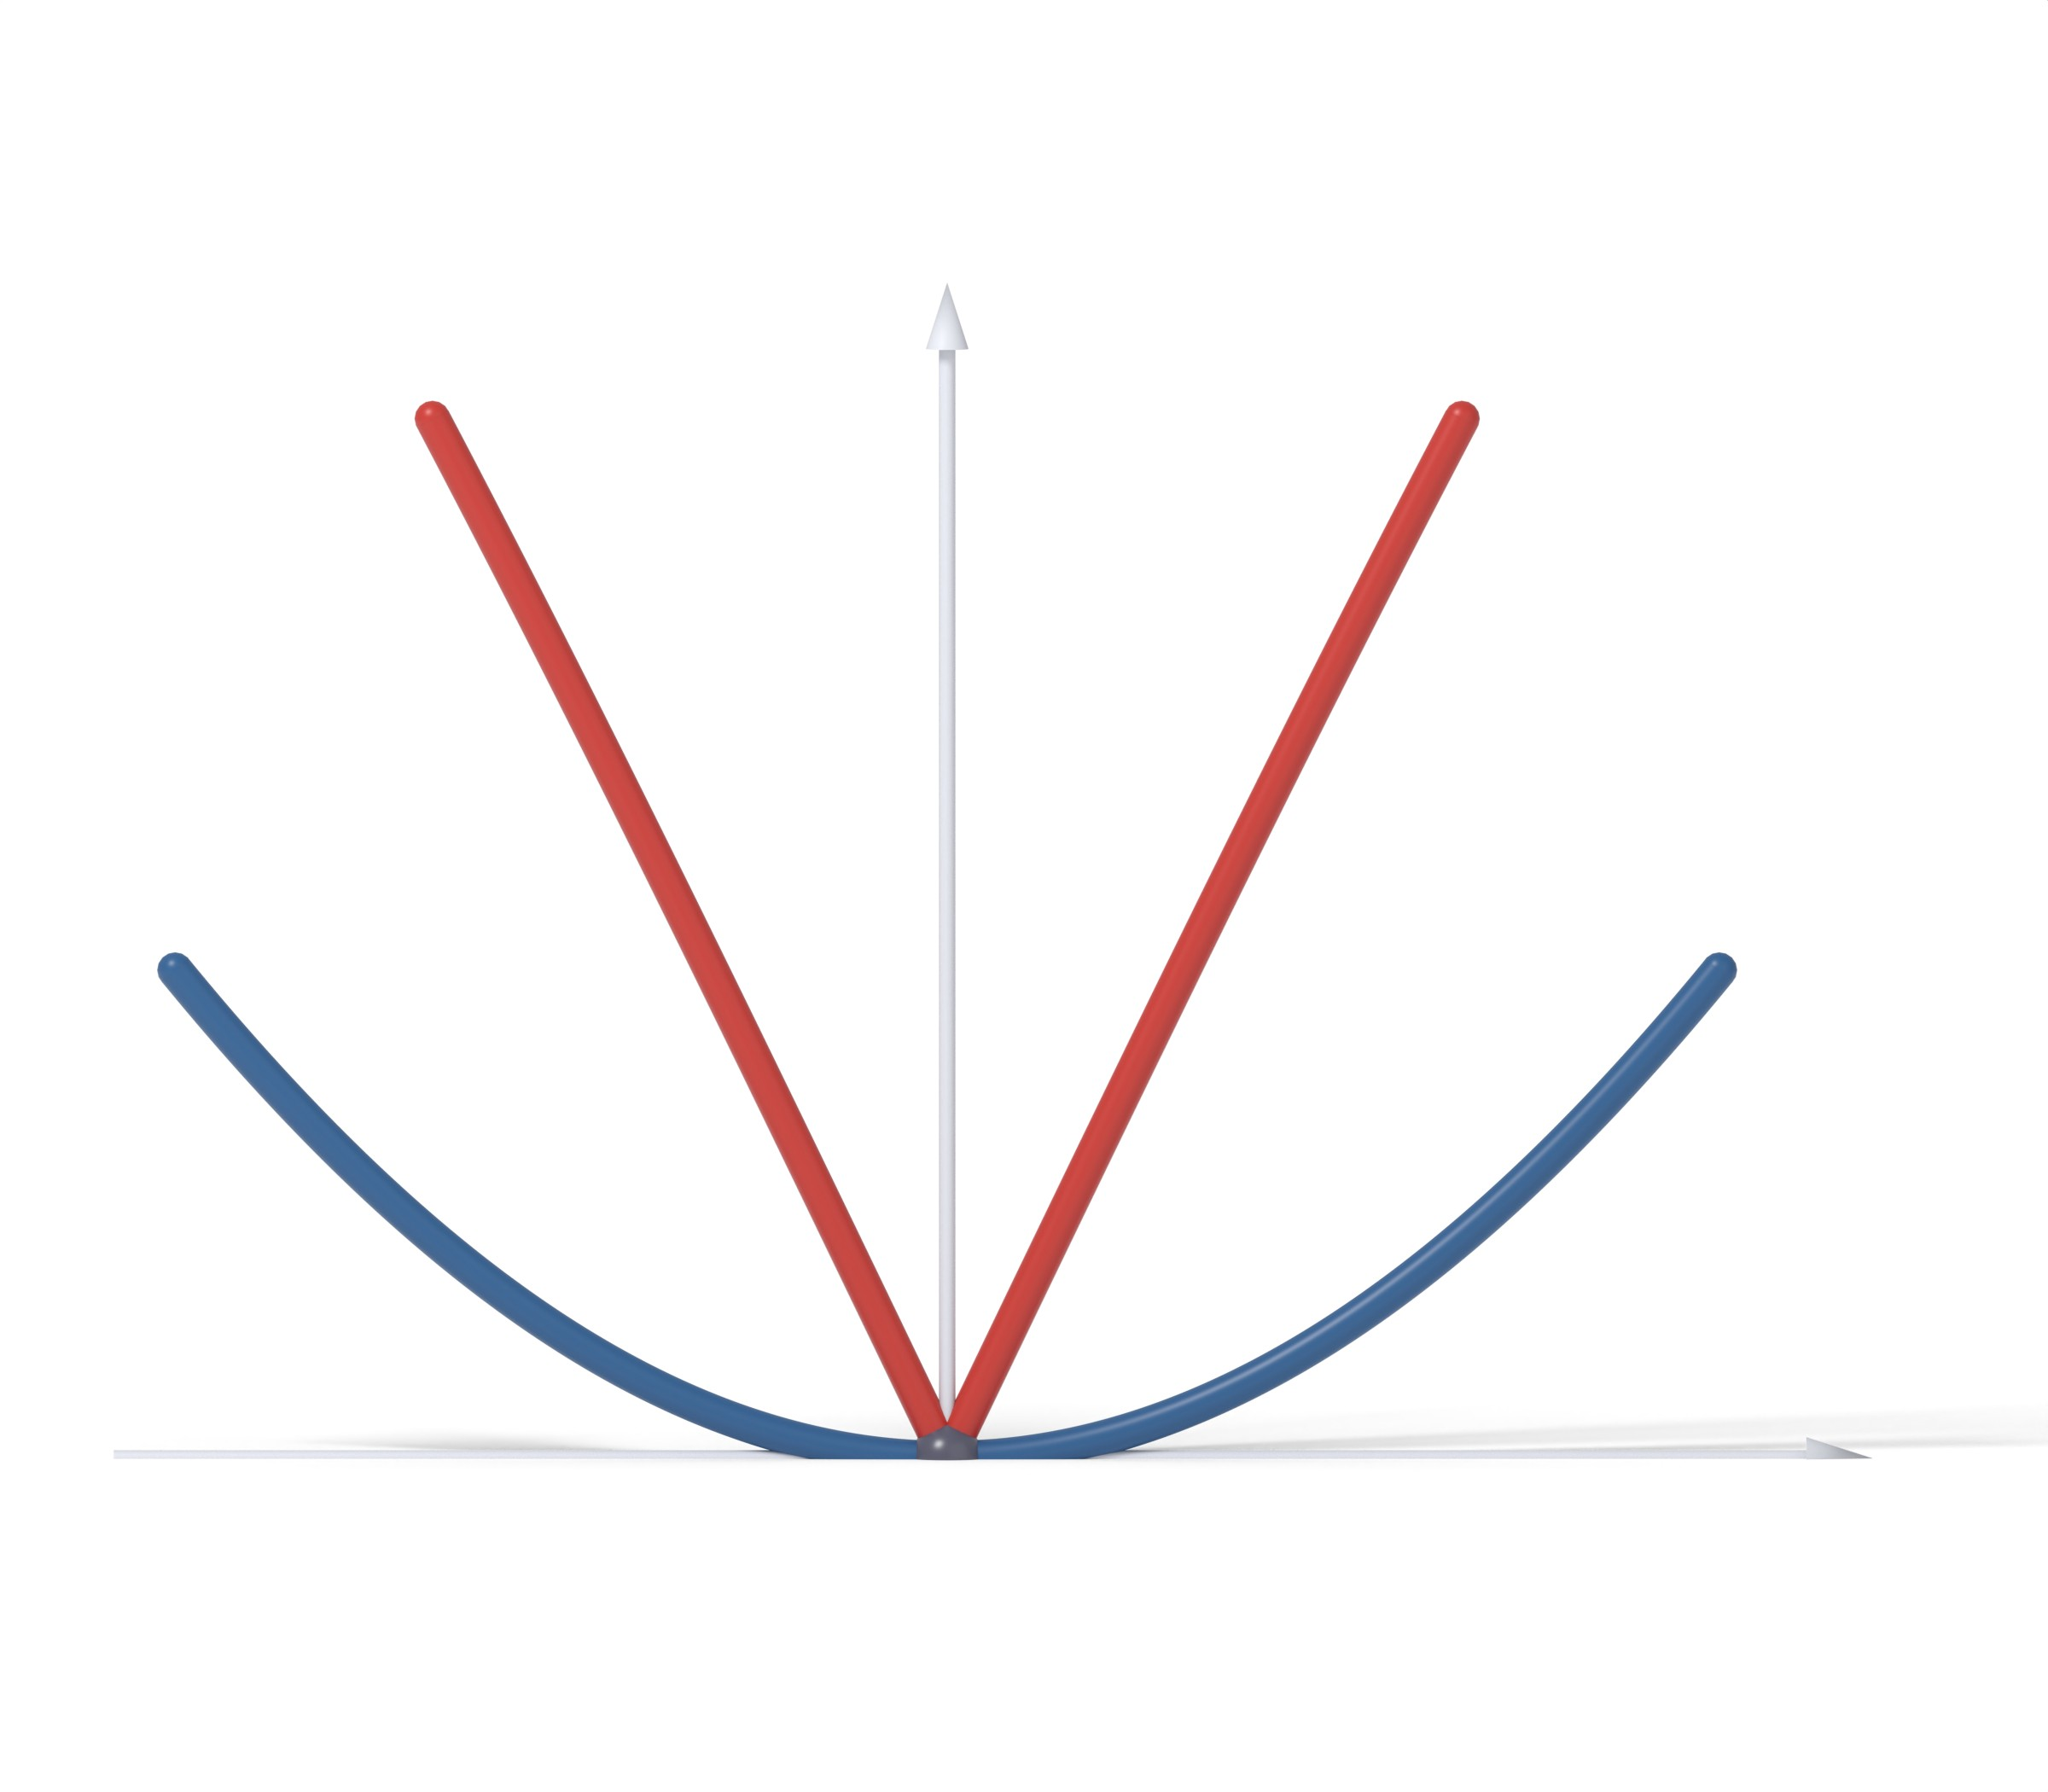
\includegraphics[width=\figw]{../blender/out/s06f06_dispersion_zoom.jpg}};
    % written by build_figure.sh; the painted part of the image
\path (0.0554\figw,0.1608\figw) rectangle (0.9988\figw,0.7371\figw);

    %% written by figlib.py; x and y in units of the image width
\coordinate (zoomk) at (0.9145\figw,0.1629\figw);
\coordinate (zoomE) at (0.4625\figw,0.7371\figw);
\coordinate (zoomkmax) at (0.8395\figw,0.1554\figw);
\coordinate (zoomkmin) at (0.0855\figw,0.1554\figw);
\coordinate (zoomfm) at (0.6962\figw,0.2564\figw);
\coordinate (zoomafm) at (0.5756\figw,0.3968\figw);
\coordinate (zoompanel) at (0.0855\figw,0.7496\figw);

    \node[lbl, anchor=north east] at (zoomk) {$ka$};
            \node[lbl, anchor=south west, text=aqmmuted] at (zoompanel) {zone centre, magnified};
  \end{scope}
\end{tikzpicture}
\end{document}
